\documentclass[a4paper, 10pt]{article}
%\usepackage{fontspec}
\usepackage[utf8]{inputenc}
\usepackage[T1]{fontenc}
\usepackage{graphicx}
\usepackage[margin=1in]{geometry}
\usepackage{hyperref}
\usepackage[french]{babel}
\usepackage[small, center]{titlesec}
\usepackage{listings}
\usepackage{float}
\usepackage{amsmath, amsthm, amssymb, mathtools}

\setlength{\parskip}{.5em}

\begin{document}
	\begin{center}
		\textbf{UE 4i900. Projet COMPLEX.}\\
		\textbf{Ordonnancement d'atelier.}\\[0.5cm]
		\textit{Alexandre Bontems, Lucas Becirspahic}
	\end{center}
	
	\section*{Partie 1 : algorithme approché avec garantie de performance}
	
	\paragraph{Question 1.}{Quelle que soit la machine M considérée, une solution optimale du problème d'ordonnancement aura un temps de résolution d'au moins $\sum_{i=1}^nd_i^M$ car il faut que toutes les tâches soient traitées sur la machine M peu importe ce qu'il ce passe sur les autres machines. Il en resulte qu'on a :
		\begin{equation*}
			OPT \geq \sum_{i=1}^nd_i^A \quad ; \quad OPT \geq \sum_{i=1}^nd_i^B \quad ; \quad OPT \geq \sum_{i=1}^nd_i^C
		\end{equation*}
          Et on en déduit une borne inférieure pour la solution optimale $OPT$:
          \begin{alignat}{2}
          	3 \times OPT &\geq \sum_{i=1}^n(d_i^A + d_i^B + d_i^C) \nonumber \\ 
          	\label{eq:3opt}
          	OPT &\geq \frac{\sum_{i=1}^n \left( d_i^A + d_i^B + d_i^C \right)}{3} 
          \end{alignat}
		Le pire des cas possibles est de n'effectuer aucune action en parallèle, donc soit $P$ une permutation quelconque, on a:
		\begin{alignat*}{2}
			P &\le \sum_{i} d_i^A + d_i^B + d_i^C \\
			P &\le 3 \times \left( \frac{1}{3} \times \sum_{i=1}^n d_i^A + d_i^B + d_i^C \right)
		\end{alignat*}
		Grâce à l'équation (\ref{eq:3opt}) on peut écrire :
		\begin{alignat*}{2}
			P &\leq 3 \times OPT \text{ donc P est 3-approché}
		\end{alignat*}}
		
	\paragraph{Question 2.}{Soit $t_J$ le temps pour les machines A et B de finir les tâches selon l'ordonnancement retourné par l'algorithme de Johnson. De plus on sait que $t_j$ est optimal pour le cas de deux machines. Soit $OPT$ le temps de réalisation d'un ordonnancement optimal sur les machines A, B et C.
          Dans notre problème on considère en plus l'exécution des tâches sur la machine $C$ donc la solution optimale $OPT$ sera supérieure ou égale à $t_J$. Ansi:
          \begin{alignat}{2}
          	\label{eq:opt_tj}
          	OPT &\geq t_j \\
          	\label{eq:opt_dic}
          	OPT &\geq \sum_{i=1}^n d_i^C
          \end{alignat}
          Soit $t^\prime_J$ le temps d'exécution de l'ordonnancement retourné par l'algorithme de Johnson sur les machines A, B et C. Dans le pire des cas, on débute les actions de la machine C à partir de $t_J$(ce cas n'arrive jamais en pratique), et donc on obtient que :
          \begin{equation*}
	          t^\prime_J \le t_J + \sum_{i=1}^n d_i^C
	      \end{equation*}
	      or d'apres (\ref{eq:opt_tj}) et (\ref{eq:opt_dic}) on obtient:
		\begin{equation*}
			t_J + \sum_{i=1}^n d_i^C \le OPT + OPT
		\end{equation*}
		On a donc un algorithme 2-approché.\\[0.35cm]
		En ce qui concerne la complexité, l'algorithme fait $n$ itérations et recherche la tâche de temps minimum sur les machines A et B ce qui se fait en $O(n)$. On a donc une complexité $O(n^2)$ pour l'algorithme de Johnson.
		}
		
	\section*{Partie 2 : méthode exacte}
		
		\paragraph{Question 4.}{On cherche ici à améliorer la borne en considérant le fait que la machine B peut être en attente de la machine A avant de commencer à traiter les tâches de l'ensemble $\pi^\prime$ (elle a fini les tâches de $\pi$ et A n'a pas finit de traiter la plus petite action de $\pi^\prime$). Ainsi, si on définit $t^{\prime\pi}_B$ tel que:
		\begin{equation*}
			t^{\prime\pi}_B = \max \left\{ t^{\pi}_B, t^{\pi}_A + \min_{i \in \pi^\prime} d^i_A \right\}
		\end{equation*}
		Lorsque $t^{\pi}_B < t^{\pi}_A + \min_{i \in \pi^\prime} d^i_A$, la machine B a fini d'exécuter les tâches de $\pi$ mais attend que la première tâche de $\pi^\prime$ soit terminée sur A pour poursuivre. Dans ce cas, le terme $t^{\prime\pi}_B$ correspond au plus petit temps avant que la machine B puisse exécuter les tâches de $\pi^\prime$. C'est pourquoi lorsqu'on remplace $t^\pi_B$ par $t^{\prime\pi}_B$ dans $b^\pi_B$ on obtient toujours une borne inférieure.\\
		
		Si on considère maintenant la machine C, on peut selon le même raisonnement définir les événements suivants:
		\begin{itemize}
			\item Lorsque $t^{\pi}_C < t^{\pi}_B + \min_{i \in \pi^\prime} d^i_B$, la machine C est en attente de la première tâche de $\pi^\prime$ sur B.
			\item Lorsque $t^\pi_C < t^\pi_A + \min_{i \in \pi^\prime} \left\{ d^i_A + d^i_B \right\}$, la machine C est en attente de la tâche la plus courte de $\pi^\prime$ sur A et B.
		\end{itemize}
		
		On peut alors remplacer $t^\pi_C$ dans $b^\pi_C$ par:
		\begin{equation*}
			t^{\prime\pi}_C = \max \left\{ t^{\pi}_C, t^{\pi}_B + \min_{i \in \pi^\prime} d^i_B,  t^\pi_A + \min_{i \in \pi^\prime} \left\{ d^i_A + d^i_B \right\} \right\}
		\end{equation*}
		}
		
		\paragraph{Question 5.}{Soit $P$ une permutation quelconque des tâches commençant par $\pi$ et $k$ une tâche de $\pi^\prime$. On peut dire que:
		\begin{enumerate}
			\item Si une action $i_1$ de $\pi^\prime$ s'exécute \textbf{avant} $k$, alors dans le meilleur des cas, elle ajoute une valeur $d^{i1}_A$ au temps total. 
			\item Si une action $i_2$ de $\pi^\prime$  s'exécute \textbf{après} $k$, alors dans le meilleur des cas, elle ajoute une valeur $d^{i2}_C$ au temps total.
		\end{enumerate}
		
		Notons maintenant $\Pi_1$ l'ensemble des tâches de $\pi^\prime$ qui s'exécutent avant $k$ et $\Pi_2$ celles qui s'exécutent après. Répartissons les tâches $i \in \pi^\prime, i \ne k$ de la manière suivante:
		\begin{itemize}
			\item si $d^i_A < d^i_C$ alors $i \in \Pi_1$,
			\item sinon $i \in \Pi_2$.
		\end{itemize}
		Cela correspond au meilleur cas possible car d'après (1) et (2), dans une version optimiste on ajoute les $d^i_A$ des tâches $\Pi_1$ et les $d^i_C$ des tâches $\Pi_2$.
		
		Il en résulte que la borne $b_2$:
		\begin{equation*}
			b_2 = \max_{k \in \pi^\prime} \left\{ t^{\pi}_A + \left(d^k_A + d^k_B + d^k_C \right) + \sum_{i \in \Pi_1} d^i_A + \sum_{i \in \Pi_2} d^i_C \right\}
		\end{equation*}
		est bien une borne inférieure du temps total pour un ordonnancement $P$ car:
		\begin{itemize}
			\item $P$ prend au moins $t^\pi_A$ unités de temps sur $\pi$,
			\item on a montré que $\left(\Pi_1, k, \Pi_2\right)$ était la meilleure façon de répartir les tâches autour de $k$ sous l'hypothèse que les tâches de $\Pi_1$ ne s'attendront pas et de même pour $\Pi_2$.
			\item De plus, on a posé aucune hypothèse sur $k$ donc dans $P$ n'importe quelle tâche de $\pi^\prime$ peut prendre le rôle de $k$.
                        \item Donc en prenant k de façon a maximiser l'expression, on est sur que quel que soit l'ordonnancement débutant par $\pi$ il sera plus grand que notre $b2$.
		\end{itemize}
		}
		
		\paragraph{Question 6.}{On pourra suivre le même raisonnement que précédemment et, en se plaçant sur les machines B et C, obtenir la borne $b_3$ suivante:
                  Répartissons les tâches $i \in \pi^\prime, i \ne k$ de la manière suivante:
		\begin{itemize}
			\item si $d^i_B < d^i_C$ alors $i \in \Pi_1$,
			\item sinon $i \in \Pi_2$.
		\begin{alignat*}{2}
			b_3 &= \max_{k \in \pi^\prime} \left\{ t^{\pi}_B + \left( d^k_B + d^k_C \right) + \sum_{i \in \Pi_1} d^i_B + \sum_{i \in \Pi_2} d^i_C \right\} \\
			b_3 &= \max_{k \in \pi^\prime} \left\{ t^{\pi}_B + \left( d^k_B + d^k_C \right) + \sum_{i \in \pi^\prime, i \ne k} \min \left\{ d^i_B, d^i_C \right\} \right\}
		\end{alignat*}
		}
		
		\paragraph{Question 8.}{On peut appliquer cette méthode arborescente et calculer les bornes quelque soit le nombre $k$ de machines. Cependant, plus on considère de machines, moins les bornes obtenues seront utiles car elles seront trop petites (trop optimistes) pour atteindre les conditions d'élaguage. 		
		}

                \paragraph{Question 10}{Nous avons mis en oeuvre un algorithme de recherche arborescente de la manière suivante : \\
                  Soit un noeud n avec un ordonnancement partiel P. Afin d'évaluer un noeud, on génère $k$ ordonnancement final débutant par P de manière aléatoire et on prend la solution la plus petite.
                  \begin{itemize}
                  \item On initialise l'algorithme avec un noeud vide(racine de l'arbre)
                  \item Tant que l'on a pas un ordonnancement final :
                  \item  A chaque étape de l'algorithme dans un noeud n, on évalue chacun de ces fils et on prend celui qui à la plus petite valeur qui devient notre noeud courant.
              

                    remarque : Pour le nombre $k$ d'évaluation d'un noeud, on choisit de prendre $k = min(borne,(taille P)!)$ de cette façon si le nombre de noeuds est suffisament petit, il les explore tous et il est limité quand on a un nombre trop important. De ce fait pour les petits ordonnancement cette alorithme retourne une solution optimal si le nombre de noeuds total < borne.

                    \begin{figure}[H]
			\centering
			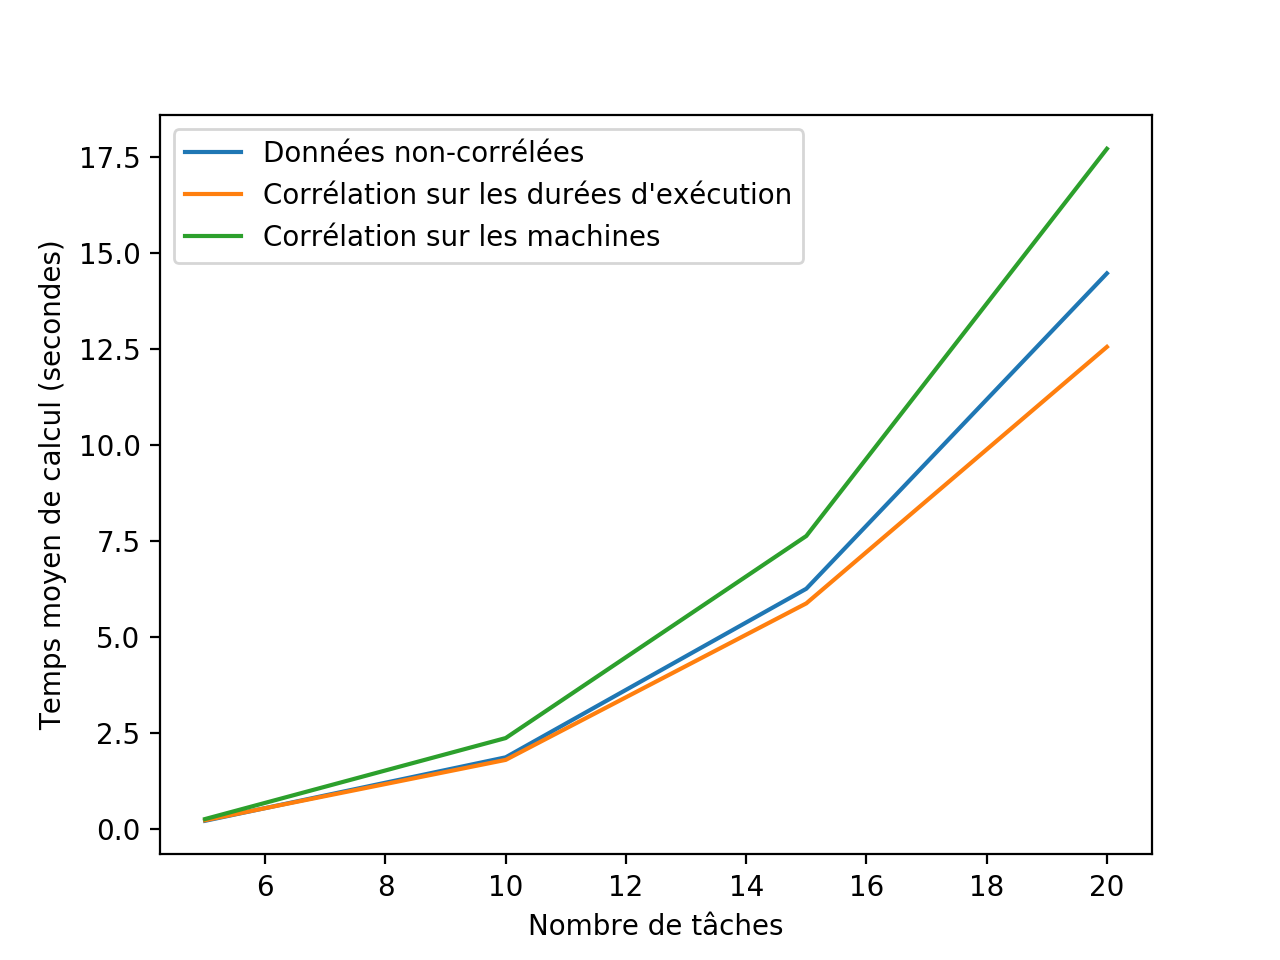
\includegraphics[width=0.85\linewidth]{graphes/branch_and_greed.png}
			\caption{Mesure de performance de l'algorithme approché avec borne=10}
			\label{fig:tj}
		\end{figure}
                    
                    }
	
	\section*{Partie 3: Mise en oeuvre}
		\subsection*{Algorithme approché}
		
		On s'intéresse tout d'abord aux performances de l'algorithme approché implémenté en Python. On observe dans la figure~\ref{fig:tj} que le temps de calcul ne varie pas selon le type de donnée ce qui est logique car la selection du max se fait en $O(n)$ peu importe la durée des tâches. De plus, on remarque que sa complexité est de $O(n^2)$ comme montré dans la partie théorique.
		
		Les données visibles en figure~\ref{fig:tj} correspondent à des moyennes de temps de résolution sur 50 instances différentes pour chaque nombre de tâches mesuré.
		
		\begin{figure}[H]
			\centering
			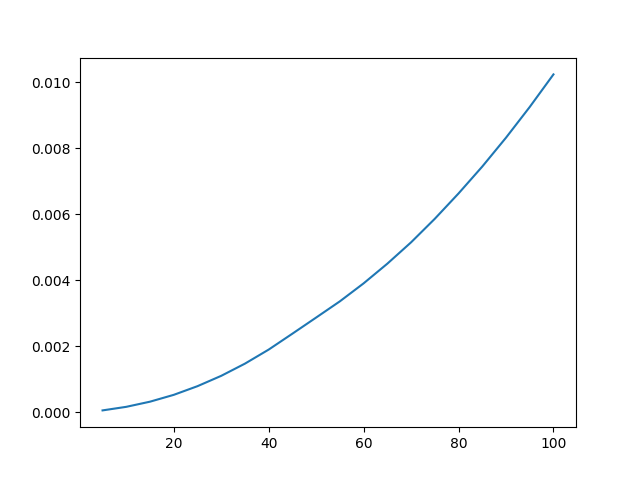
\includegraphics[width=0.85\linewidth]{graphes/Johnson.png}
			\caption{Mesure de performance de l'algorithme Johnson}
			\label{fig:tj}
		\end{figure}

                Pour verifier que la complexité est bien $O(n^2)$ on procède de la manière suivante : on fait l'hypothèse que nous avons une fonction polynomiale de la forme $f(x) = \lambda x^p$ avec $\lambda$ et p appartenant à R.
                De ce fait en passant au log on obtient : $log(f(x)) = log(\lambda) + p*log(x)$ avec $log(\lambda)$ une constante. De ce fait en tracant x : log(x), y :log(f(x)) et en calculant la pente on obtient p, c'est à dire la puissance de notre polynome.

                \begin{figure}[H]
			\centering
			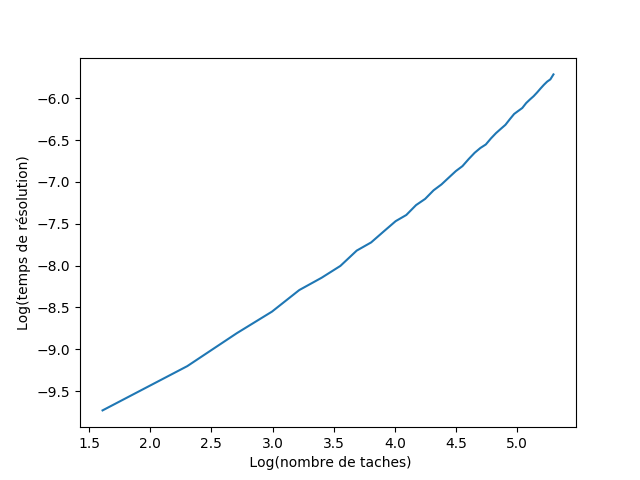
\includegraphics[width=0.8\linewidth]{graphes/verification_Johnson.png}
			\caption{Verification de la complexité}
			\label{fig:??}
		\end{figure}
                En procédant ainsi on obtient p = 1.14227148219, ce qui est contraire à notre afirmation théorique. Cela peut être du à la façon de trouver le plus petit element de la matrices des taches par numpy qui est optimisé .
                
		
		\begin{figure}[H]
			\centering
			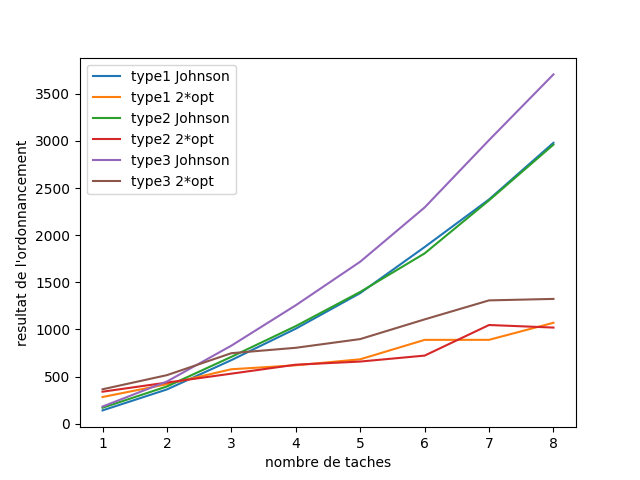
\includegraphics[width=0.8\linewidth]{graphes/verifValiditeJohnson.png}
			\caption{Verification de la validité de Johnson}
			\label{fig:validiteJ}
		\end{figure}
                
		
		Pour vérifier que nos algorithmes approchés retournent le bon résultat on trace leur resultat et 2*opt pour tous les types de donnés. La figure est fausse car 500 temps pour 1 tache est abérent (figure~\ref{fig:validiteJ}).
		
		\subsection*{Méthode exacte}
		
	L'algorithme correspondant à la méthode arborescente a été implémenté en Python. Pour mesurer ses performances, on a d'abord mesuré le temps de résolution moyen pour des instances de taille croissante comme pour Johnson. Cela étant, les temps de résolution étant particulièrement longs pour des grandes instances, on borne le nombre maximal de tâches à 6. La figure~\ref{fig:temps_exact} présente les mesures réalisées avec les bornes inférieures $b_1$ et $\max\left\{ b_1, b_2, b_3 \right\}$ étudiées en partie théorique.
		
		\begin{figure}[h]
			\centering
			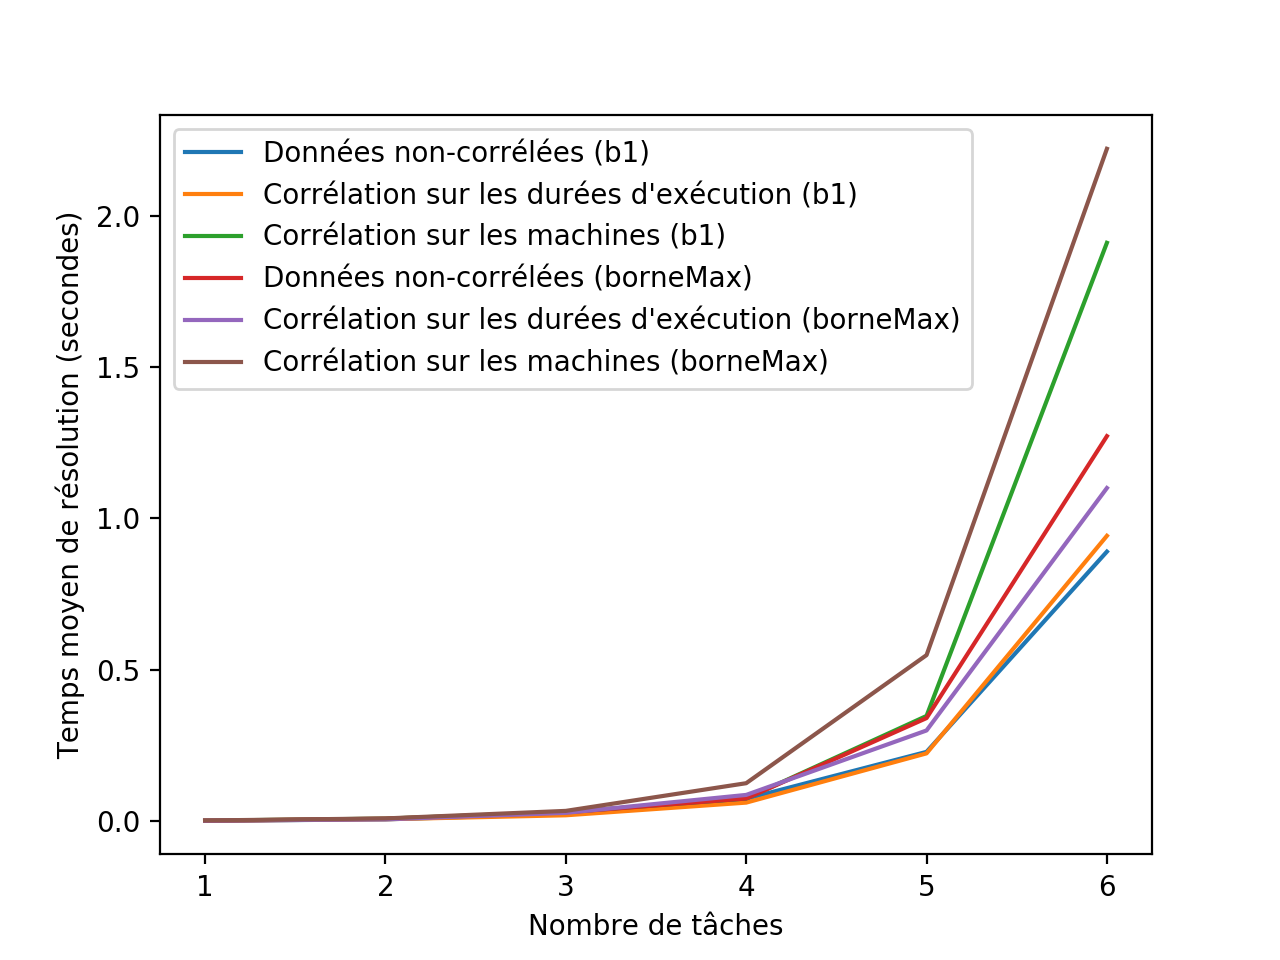
\includegraphics[width=0.85\linewidth]{graphes/time_exact_20iter_b1bmax.png}
			\caption{Mesure de performance de la méthode arborescente}
			\label{fig:temps_exact}
		\end{figure}
		
	On remarque, dans la figure~\ref{fig:temps_exact}, que le temps de calcul pour les données avec corrélation sur machines est nettement plus important que pour les autres. Cela s'explique par le fait que durées les plus longues sont situées sur la machine C. De ce fait la borne $b^\pi_A$ de $b_1$ est trop optimiste donc ne va pas être prise par le max ($b_1 = \max\left\{b^\pi_A, b^\pi_B, b^\pi_C\right\}$), de meme pour la borne $b^\pi_B$. Il reste uniquement la borne $b^\pi_C$ qui devient réaliste seulement que l'ordonnancement $\pi$ est grand donc il faut explorer l'arbre en profondeur afin d'avoir des élagages ce qui explique que la lenteur de l'algorithme pour ce type de données.
		
		\paragraph{Notes expérimentales}{Il semble que la borne $b_2$ retourne une valeur plus faible de manière générale, de ce fait on coupe moins de noeuds avec cette borne. En revanche, elle est plus rapide à calculer. Sur l'exemple test3, avec la borne b2 on explore 87 pourcent de l'arbre alors que la borne b1 nous fait exploré 76 pourcent de l'arbre. \\
                  Soit n le nombre de taches.
                  Dans les algorithmes de la partie exacte, à chaque niveau k de l'arbre on a un ordonnancement de taille k (sauf pour le niveau 0 ou on a juste 1 noeud). Dans chaque ordonnancement la première tache à n valeurs possibles la seconde n-1 et ainsi de suite. Par exemple pour un ordonnancement de taille 3 on a : 1(racine) + 3 + 3*2 + 3*2*1 = 16 noeuds. Le nombre de noeud est exponentiellement grand. De ce fait on prendra uniquement des instances de taille 9 maximum. \\
                  Le choix de la solution initiale comme borne est très important et peut réduire considérablement le temps de calcul.
                }
                \paragraph{graphes et observations}{

                  Dans ce projet on utilisera type1 pour designer les données non-corrélées, type2 pour les corrélation sur les durées d'exécution et type3 pour corrélation sur les machines.\\

                  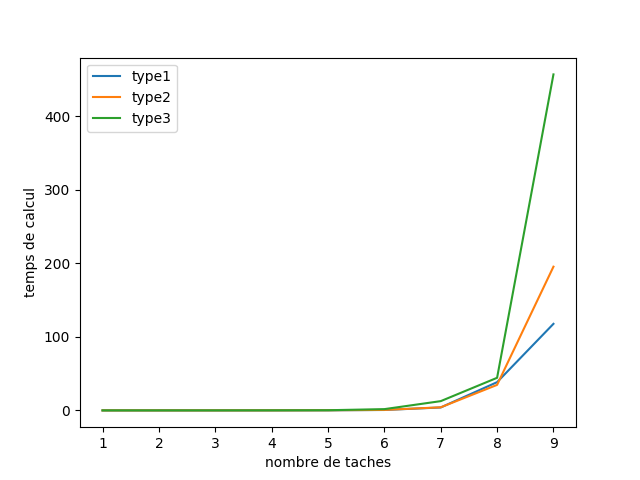
\includegraphics{graphes/exacte_b1.png}
                  
                  
                }
                \paragraph{}{
                  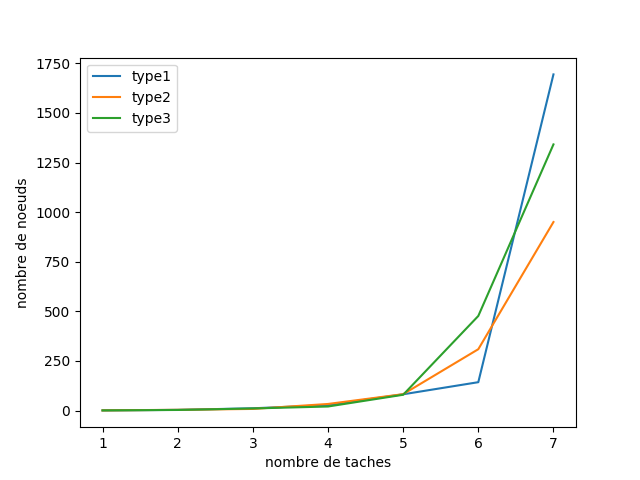
\includegraphics{graphes/node_b1.png}
                  Nombre de noeuds explorés par la methode exacte avec la borne b1. On observe que le type1 explore le plus de noeud alors que les données de ce type sont les plus rapides à calculer(voir graphe au dessus).
                  On peut donc supposer que les bornes sont plus rapides à calculer ?
                }

                \paragraph{}{
                  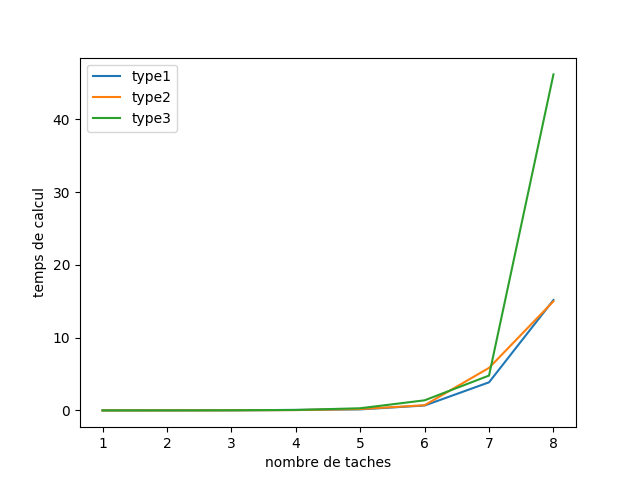
\includegraphics{graphes/exact_b2.png}
                  La methode arborescente avec la borne b2. On remarque que la borne b2 à un meilleur temps de calcul bien qu'elle coupe moins de noeuds. C'est lié au fait qu'elle est plus rapide à calculer.
                }

                \paragraph{}{
                  Soit methode1 , la methode arborescente en initialisant la borne supérieur à $\inf$.
                  Soit methode2 , la methode arborescente en initialisant la borne supérieur avec le résultat de l'algorithme de Johnson
                  
                  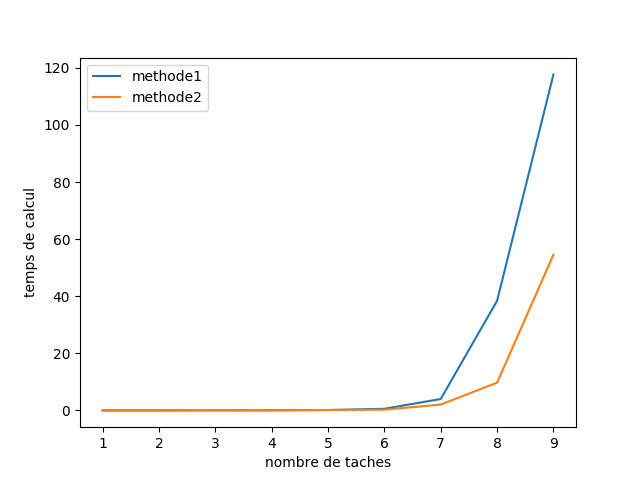
\includegraphics{graphes/exacte_vs_mix_type1.png}
                  }
                Pour le type 1
                \paragraph{}{
                  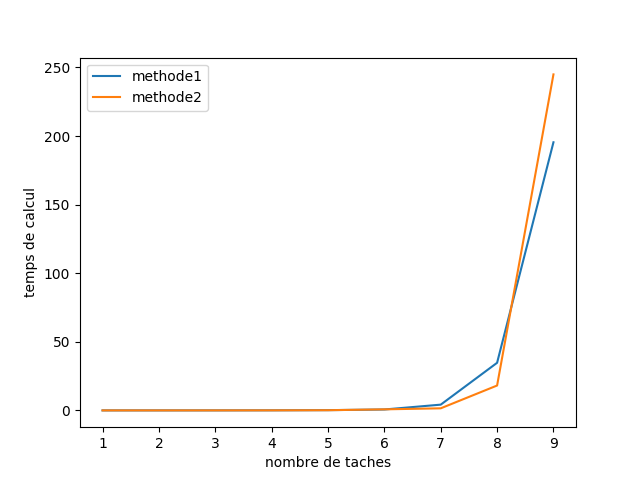
\includegraphics{graphes/exact_vs_mix_type2.png}
                  Pour le type 2
                }
                \paragraph{}{
                  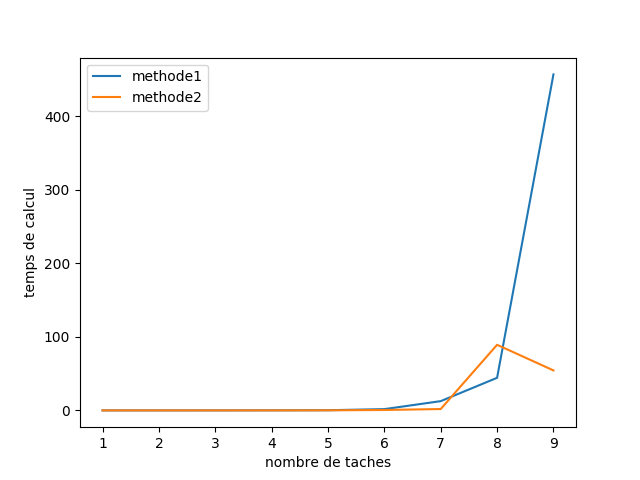
\includegraphics{graphes/exact_vs_mix_type3.png}
                  Pour le type 3
                }
                  
\end{document}
